%%%%%%%%%%%%%%%%%%%%%%%%%%%%%%%%%%%%%%%%%

%%%%%%%%%%%%%%%%%%%%%%%%%%%%%%%%%%%%%%%%%

%----------------------------------------------------------------------------------------
%	PACKAGES AND DOCUMENT CONFIGURATIONS
%----------------------------------------------------------------------------------------

\documentclass[https://www.overleaf.com/project/63761df255a8a9f4a15c3579
	letterpaper, % Paper size, specify a4paper (A4) or letterpaper (US letter)
	10pt, % Default font size, specify 10pt, 11pt or 12pt
]{CSUniSchoolLabReport}



\usepackage[normalem]{ulem}
\usepackage{listings}
\usepackage{xcolor}
\definecolor{codegreen}{rgb}{0,0.6,0}
\definecolor{codegray}{rgb}{0.5,0.5,0.5}
\definecolor{codepurple}{rgb}{0.58,0,0.82}
\definecolor{backcolour}{rgb}{1,1,1}
\lstdefinestyle{mystyle}{
    backgroundcolor=\color{backcolour},   
    commentstyle=\color{codegreen},
    keywordstyle=\color{magenta},
    numberstyle=\tiny\color{codegray},
    stringstyle=\color{codepurple},
    basicstyle=\ttfamily\footnotesize,
    breakatwhitespace=false,         
    breaklines=true,                 
    captionpos=b,                    
    keepspaces=true,                 
    numbers=left,                    
    numbersep=5pt,                  
    showspaces=false,                
    showstringspaces=false,
    showtabs=false,                  
    tabsize=2
}

\lstset{style=mystyle}
\renewcommand\ULthickness{1.0pt}   %%---> For changing thickness of underline
\setlength\ULdepth{1.3ex}%\maxdimen ---> For changing depth of underline

%----------------------------------------------------------------------------------------
%	REPORT INFORMATION
%----------------------------------------------------------------------------------------


\begin{document}

\begin{figure}[H] % [H] forces the figure to be placed exactly where it appears in the text
	\centering % Horizontally center the figure
	
\includegraphics[width=0.4\textwidth]{Figures/logo.png} % Include the figure
\end{figure}

\begin{center}
	\begin{tabular} {c}
        \Huge Universidad La Salle \\\\\\\\
		\huge Fundamentos de Lenguajes de Programación \\\\\\\\
		\LARGE Informe \\\\\\\\
        \huge Una Comparación entre C++, Go y Python \\\\\\\\
        \LARGE Karlo Emigdio Pacha Curimayhua \\\\\\\\
        \LARGE Quinto Semestre - Ingeniería de Software \\\\\\\\
		\LARGE 2022
	\end{tabular}
\end{center}

\begin{center}
	\begin{tabular}{l r}
	\end{tabular}
\end{center}



% If you need to include an abstract, uncomment the lines below
%\begin{abstract}
%	Abstract text
%\end{abstract}

%----------------------------------------------------------------------------------------
%	Introducción
%----------------------------------------------------------------------------------------

\section{Introducción}

Go es un lenguaje de programación compilado basado en C (en el aspecto sintáctico) y parecido a Python al momento del dinamismo que posee. El objetivo de este trabajo es poner a prueba los 3 lenguajes mencionados con los algoritmos de ordenamiento: Cocktail Sort y Counting Sort.
 
%----------------------------------------------------------------------------------------
%	Algoritmos
%----------------------------------------------------------------------------------------

\section{Algoritmos}

\subsection{Cocktail Sort}

Es un algoritmo de ordenamiento con complejidad cuadrática \(O(n^2)\) como se puede apreciar en la Tabla 1; este es una variación del Bubble Sort que recorre la lista de datos en ambas direcciones de forma alternativa (al contrario que el Bubble Sort que sólo lo hace en una dirección). \\
Los pasos son:\\

\begin{center}
    \begin{tabular}{| c | c |}
        \hline
            Caso & Complejidad \\ 
        \hline
            Mejor caso & \(O(n)\) \\
            Caso promedio & \(O(n^2)\) \\
            Peor caso & \(O(n^2)\) \\ 
        \hline
    \end{tabular}
\end{center}

 \begin{center}
    Tabla 1 : Complejidad Temporal
 \end{center}

\begin{tabular}{lr}
    I. El primer paso es recorrer la lista de datos de izquierda a derecha, se comparan \\
    los valores adyacentes, y si el valor de la izquierda es mayor, se intercambian los \\
    valores. El objetivo es poner el valor máximo al final.\\\\

    II. El segundo paso es recorrer la lista de datos de derecha a izquierda, se \\
    comparan los valores adyacentes, y si el valor de la derecha es menor, se intercambi-\\
    an los valores. El objetivo es poner el valor mínimo al inicio.\\\\
\end{tabular}

Este proceso continúa hasta que los elementos de la matriz no se ordenan.\\


\subsection{Counting Sort}

Es un algoritmo de ordenamiento con complejidad  \(O(n + k)\), esta aplica para todos los casos como se puede apreciar en la Tabla 2; este algoritmo basa su funcionamiento en los índices, no en comparaciones como los demás. Este algoritmo depende mucho del elemento con el valor máximo. \\


\begin{center}
    \begin{tabular}{| c | c |}
        \hline
            Caso & Complejidad \\ 
        \hline
            Mejor caso & \(O(n + k)\) \\
            Caso promedio & \(O(n + k)\) \\
            Peor caso & \(O(n + k)\) \\ 
        \hline
    \end{tabular}
\end{center}

 \begin{center}
    Tabla 2 : Complejidad Temporal
 \end{center}

Los pasos son:\\

\begin{tabular}{lr}
    I. Busca el elemento máximo (max) y el mínimo (min).\\\\
    II. Crea una lista auxiliar de tamaño max + 1.\\\\
    III. Se subdivide en los siguientes pasos:\\\\
    \begin{tabular}{lr}
        - Se almacena el recuento de cada elemento de la lista en su índice correspon-\\
        diente en la lista auxiliar.\\\\
        - Se suman los recuentos (a[i] + a[i-1]]), esto para colocar los elementos en \\
        el índice correcto de la lista ordenada.\\\\
    \end{tabular}
    \\IV. Posiciona los elementos en la lista original o una de salida, para esto se utilizan los índices.\\\\
\end{tabular}

El punto débil de este algoritmo es la complejidad espacial O(max), si el elemnto de mayor valor tiene un número de dígidos superior al tamaño de la lista de datos, el costo es casi cuadrático.\\


%----------------------------------------------------------------------------------------
%	Implementación
%----------------------------------------------------------------------------------------

\section{Implementación}

Para poner a prueba los algoritmos de Cocktail y Counting Sort, se necesitan varios archivos CSV que contengan entre: 100, 1000, 2000, 3000, 4000, 5000, 6000, 7000, 8000, 9000, 10000, 20000, 30000, 40000 y 50000 datos. \\\\
Una vez se implementen los algoritmos en los 3 lenguajes, se ejecutarán con cada lista de datos generada, por cada tamaño se ejecutará y medirá el tiempo de ejecició (en segundos) 5 veces y luego se obtendrá un promedio. \\\\
Finalmente, los datos obtenidos se exportarán en un CVS.

\subsection{Generador C++}
\lstinputlisting[language=Octave]{codes/generator.cpp}

\subsection{Cocktail Sort C++}
\lstinputlisting[language=Octave]{codes/CocktailSort.cpp}

\subsection{Cocktail Sort Go}
\lstinputlisting[language=Octave]{codes/CocktailSort.go}

\subsection{Cocktail Sort Python}
\lstinputlisting[language=Octave]{codes/CocktailSort.py}

\subsection{Counting Sort C++}
\lstinputlisting[language=Octave]{codes/CountingSort.cpp}

\subsection{Counting Sort Go}
\lstinputlisting[language=Octave]{codes/CountingSort.go}

\subsection{Counting Sort Python}
\lstinputlisting[language=Octave]{codes/CountingSort.py}

\subsection{Graficador Python}
\lstinputlisting[language=Octave]{codes/grapher.py}

%----------------------------------------------------------------------------------------
%	Resultados
%----------------------------------------------------------------------------------------

\section{Resultados}

\subsection{Graficador Python}

\subsection{Cocktail Sort}

\begin{figure}[H] 
	\centering 
	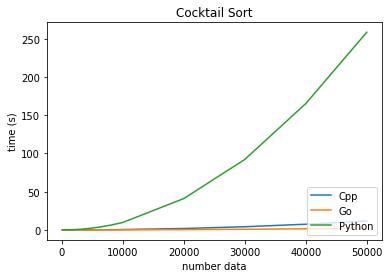
\includegraphics[width=0.9\textwidth]{Figures/cocktailSort.png} % Include the figure
	\caption{Cocktail Sort en C++, Go y Python}
\end{figure}

\begin{figure}[H] 
	\centering 
	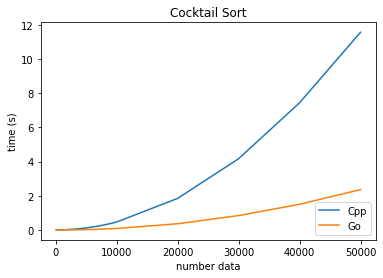
\includegraphics[width=0.8\textwidth]{Figures/cocktailSort2.png} % Include the figure
	\caption{Cocktail Sort en C++ y Go}
\end{figure}


\subsection{Counting Sort}

\begin{figure}[H] 
	\centering 
	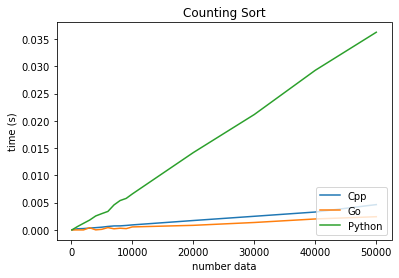
\includegraphics[width=0.8\textwidth]{Figures/countingSort.png} % Include the figure
	\caption{Counting Sort en C++, Go y Python}
\end{figure}

\begin{figure}[H] 
	\centering 
	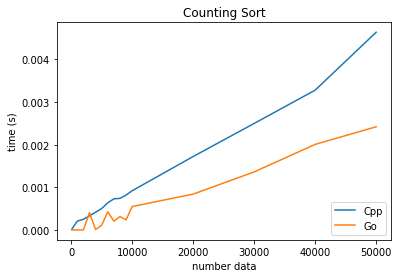
\includegraphics[width=0.9\textwidth]{Figures/countingSort2.png} % Include the figure
	\caption{Counting Sort en C++ y Go}
\end{figure}

%----------------------------------------------------------------------------------------
%	DISCUSSION
%----------------------------------------------------------------------------------------

\section{Discussion of Experimental Uncertainty}

The accepted value (periodic table) is \SI{24.3}{\gram\per\mole} \autocite{Smith:2022qr}. The percentage discrepancy between the accepted value and the result obtained here is 1.3\%. Because only a single measurement was made, it is not possible to calculate an estimated standard deviation (see \textcite{Smith:2021jd}).

The most obvious source of experimental uncertainty is the limited precision of the balance. Other potential sources of experimental uncertainty are: the reaction might not be complete; if not enough time was allowed for total oxidation, less than complete oxidation of the magnesium might have, in part, reacted with nitrogen in the air (incorrect reaction); the magnesium oxide might have absorbed water from the air, and thus weigh ``too much." Because the result obtained is close to the accepted value it is possible that some of these experimental uncertainties have fortuitously cancelled one another.

%----------------------------------------------------------------------------------------
%	ANSWERS TO DEFINITIONS
%----------------------------------------------------------------------------------------

\section{Answers to Definitions}

\begin{enumerate}
	\item The \textit{atomic weight of an element} is the relative weight of one of its atoms compared to C-12 with a weight of 12.0000000$\ldots$, hydrogen with a weight of 1.008, to oxygen with a weight of 16.00. Atomic weight is also the average weight of all the atoms of that element as they occur in nature.
	\item The \textit{units of atomic weight} are two-fold, with an identical numerical value. They are g/mole of atoms (or just g/mol) or amu/atom.
	\item \textit{Percentage discrepancy} between an accepted (literature) value and an experimental value is:
		\begin{equation*}
			\frac{\mathrm{experimental\;result} - \mathrm{accepted\;result}}{\mathrm{accepted\;result}}
		\end{equation*}
\end{enumerate}

%----------------------------------------------------------------------------------------
%	BIBLIOGRAPHY
%----------------------------------------------------------------------------------------

\printbibliography % Output the bibliography

%----------------------------------------------------------------------------------------

\end{document}